\section{矩阵光学}
\subsection{综述}
对任意理想光具组，选定前后变换面后，其对傍轴光线的作用一定可以写为：
\begin{equation}
	\begin{pmatrix}
		y' \\ \alpha'
	\end{pmatrix}
	=
	\begin{pmatrix}
		a & b \\
		c & d
	\end{pmatrix}
	\begin{pmatrix}
		y \\ \alpha
	\end{pmatrix}=
	M\begin{pmatrix}
		y \\ \alpha
	\end{pmatrix}.
\end{equation}
其中，\(y\) 与 \(y'\) 分别为前、后变换面处光线离光轴的距离，\(\alpha\) 与 \(\alpha'\) 为前、后变换面处光线与光轴的夹角，且 \(\alpha,\alpha'\ll1\).

例如，在均匀介质中传播距离 \(L\) 时，对应矩阵
\begin{equation*}
	M_{\mathrm{freespace}} = \begin{pmatrix}
		1 & L \\
		0 & 1
	\end{pmatrix}.
\end{equation*}

例如，被曲率半径为 \(r\) 的球面折射（\(r>0\)则凸向\(n_1\)一侧）时，对应矩阵
\begin{equation*}
	M_{\mathrm{sphere}} = \begin{pmatrix}
		1                         & 0                \\
		\dfrac{n_1 - n_2}{n_2\,r} & \dfrac{n_1}{n_2}
	\end{pmatrix}.
\end{equation*}

例如，物方焦距为 \(f\)、像方焦距为 \(f'\) 的薄透镜，从其物方主面 \(H\) 到像方主面 \(H'\) 的传播矩阵为
\begin{equation}
	M_{HH'} = \begin{pmatrix}
		1              & 0             \\
		-\dfrac{1}{f'} & \dfrac{f}{f'}
	\end{pmatrix}.
\end{equation}
从其物方节点 \(N\) 到像方节点 \(N'\) 的传播矩阵为
\begin{equation}
	M_{NN'} = \begin{pmatrix}
		\alpha & 0 \\
		\beta  & 1
	\end{pmatrix},\quad\text{其中 \(\alpha, \beta\) 为任意常数.}
\end{equation}


记光具组 \(M\) 的物方主面距前变换面的距离为 \(h\)，物方节点距前变换面距离为 \(p\)，物方焦点距物方主面距离为 \(f\)，如图\ref{主面节点焦点图}，图中 \(h,p,f>0\).

实际上，任意一组前后变换面均可等价为由一组主面、一组节点、两个焦点组成的类薄透镜系统.

证明如下：

考虑变换面前\(z\)面到后\(z'\)面的变换矩阵
\begin{equation*}
	M=\begin{pmatrix}
		1 & z' \\
		0 & 1
	\end{pmatrix}
	\begin{pmatrix}
		a & b \\
		c & d
	\end{pmatrix}
	\begin{pmatrix}
		1 & z \\
		0 & 1
	\end{pmatrix}
	=
	\begin{pmatrix}
		a + c z' & a z + b + z'\,(c z + d) \\
		c        & c z + d
	\end{pmatrix}.
\end{equation*}

若令其具有物方主面变换至像方主面
\begin{equation*}
	\text{}\quad
	M_{HH'}=\begin{pmatrix}
		1              & 0             \\
		-\dfrac{1}{f'} & \dfrac{f}{f'}
	\end{pmatrix}
\end{equation*}
的形式，并记此时的\(z=h,z'=h',\)解得：
\begin{align}
	h' & = \dfrac{1 - a}{c}, \quad h  = \dfrac{a d - b c - d}{c}, \\
	f' & = -\dfrac{1}{c}, \quad f  = -\dfrac{a d - b c}{c},       \\
	M  & =M_{HH'} =
	\begin{pmatrix}
		1 & 0         \\
		c & a d - b c
	\end{pmatrix}
	=
	\begin{pmatrix}
		1              & 0             \\
		-\dfrac{1}{f'} & \dfrac{f}{f'}
	\end{pmatrix}.
\end{align}

若令其具有物方节点变换到像方节点
\begin{equation*}
	\text{}\quad
	M_{NN'}=\begin{pmatrix}
		\alpha & 0 \\
		\beta  & 1
	\end{pmatrix}
\end{equation*}
的形式，并记此时的\(z=p,z'=p',\)解得：
\begin{align}
	p' & = \dfrac{a d - b c - a}{c}, \quad p  = \dfrac{1 - d}{c}, \\
	M  & =M_{NN'} =
	\begin{pmatrix}
		a d - b c & 0 \\
		c         & 1
	\end{pmatrix}.
\end{align}

以上几条式子既证明了原结论，还直接给出了焦点、节点位置与变换矩阵矩阵元的关系.

\subsection{透镜的变换矩阵}
下举几个变换矩阵矩阵元实例.

1.双薄透镜光具组
\begin{equation*}
	\begin{pmatrix}a & b \\ c & d\end{pmatrix}
	=
	\begin{pmatrix}
		1                & 0                 \\[6pt]
		-\dfrac{1}{f_2'} & \dfrac{f_2}{f_2'}
	\end{pmatrix}
	\begin{pmatrix}
		1 & \Delta + f_1' + f_2 \\[6pt]
		0 & 1
	\end{pmatrix}
	\begin{pmatrix}
		1                & 0                 \\[6pt]
		-\dfrac{1}{f_1'} & \dfrac{f_1}{f_1'}
	\end{pmatrix},\\
\end{equation*}
\begin{align*}
	a & = -\dfrac{\Delta + f_2}{f_1'},
	\quad b = \dfrac{f_1}{f_1'}\bigl(\Delta + f_1' + f_2\bigr), \\
	c & = \dfrac{\Delta}{f_1' f_2'},
	\quad d = -\dfrac{(\Delta + f_1')\,f_1}{f_1' f_2'},\quad ad - bc = \dfrac{f_1 f_2}{f_1' f_2'}.
\end{align*}

2.三薄透镜光具组：
\begin{equation*}
	\begin{pmatrix}a & b \\ c & d\end{pmatrix}
	=
	\begin{pmatrix}
		1                & 0                 \\[4pt]
		-\dfrac{1}{f_3'} & \dfrac{f_3}{f_3'}
	\end{pmatrix}
	\begin{pmatrix}
		1 & \Delta_2 + f_2' + f_3 \\[4pt]
		0 & 1
	\end{pmatrix}
	\begin{pmatrix}
		1                & 0                 \\[4pt]
		-\dfrac{1}{f_2'} & \dfrac{f_2}{f_2'}
	\end{pmatrix}
	\begin{pmatrix}
		1 & \Delta_1 + f_1' + f_2 \\[4pt]
		0 & 1
	\end{pmatrix}
	\begin{pmatrix}
		1                & 0                 \\[4pt]
		-\dfrac{1}{f_1'} & \dfrac{f_1}{f_1'}
	\end{pmatrix}
\end{equation*}
\begin{align*}
	a & = \dfrac{\Delta_1\Delta_2 + \Delta_1 f_3 - f_2 f_2'}{f_1' f_2'},
	\quad b = \dfrac{f_1}{f_1' f_2'}\Bigl(f_2 f_2' - \Delta_1\Delta_2 - \Delta_1 f_3 - f_1'\Delta_2 - f_1' f_3\Bigr), \\
	c & = \dfrac{f_2 f_2' - \Delta_1\Delta_2}{f_1' f_2' f_3'},
	\quad d = \dfrac{f_1}{f_1' f_2' f_3'}\Bigl(-f_2 f_2' + \Delta_1\Delta_2 + f_1'\Delta_2\Bigr),\quad ad - bc = \dfrac{f_1 f_2 f_3}{f_1' f_2' f_3'}.
\end{align*}

3.四薄透镜光具组：
\begin{align*}
	\begin{pmatrix}a & b \\ c & d\end{pmatrix}
	  & =
	\begin{pmatrix}
		1                & 0                 \\[4pt]
		-\dfrac{1}{f_4'} & \dfrac{f_4}{f_4'}
	\end{pmatrix}
	\begin{pmatrix}
		1 & \Delta_3 + f_3' + f_4 \\[4pt]
		0 & 1
	\end{pmatrix}
	\begin{pmatrix}
		1                & 0                 \\[4pt]
		-\dfrac{1}{f_3'} & \dfrac{f_3}{f_3'}
	\end{pmatrix}                                                                                                \\
	  & \begin{pmatrix}
		    1 & \Delta_2 + f_2' + f_3 \\[4pt]
		    0 & 1
	    \end{pmatrix}
	\begin{pmatrix}
		1                & 0                 \\[4pt]
		-\dfrac{1}{f_2'} & \dfrac{f_2}{f_2'}
	\end{pmatrix}
	\begin{pmatrix}
		1 & \Delta_1 + f_1' + f_2 \\[4pt]
		0 & 1
	\end{pmatrix}
	\begin{pmatrix}
		1                & 0                 \\[4pt]
		-\dfrac{1}{f_1'} & \dfrac{f_1}{f_1'}
	\end{pmatrix}                                                                                                \\
	a & = \dfrac{1}{f_1' f_2' f_3'}\Bigl(\Delta_1 f_3 f_3' + (\Delta_3 + f_4)\,(f_2 f_2' - \Delta_1\Delta_2)\Bigr),                            \\
	b & = \dfrac{f_1}{f_1' f_2' f_3'}\Bigl(-f_3 f_3'(\Delta_1 + f_1') + (\Delta_3 + f_4)\,(-f_2 f_2' + \Delta_1\Delta_2 + f_1'\Delta_2)\Bigr), \\
	c & = -\dfrac{1}{f_1' f_2' f_3' f_4'}\Bigl(\Delta_1 f_3 f_3' + \Delta_3 f_2 f_2' - \Delta_1\Delta_2\Delta_3\Bigr),                         \\
	d & = \dfrac{f_1}{f_1' f_2' f_3' f_4'}\Bigl(f_3 f_3'(\Delta_1 + f_1') - \Delta_3\,(-f_2 f_2' + \Delta_1\Delta_2 + f_1'\Delta_2)\Bigr),     \\
	  & ad - bc = \dfrac{f_1 f_2 f_3 f_4}{f_1' f_2' f_3' f_4'}.
\end{align*}
\subsection{高斯光束的变换}
在柱坐标下，高斯光束的振幅随空间变化为
\begin{equation}
	U(r,z)
	=U_0\,\dfrac{\omega_0}{\omega(z)}
	\exp\bigl[-\dfrac{r^2}{\omega(z)^2}\bigr]
	\exp\bigl[\mathrm{i}k\bigl(z+\dfrac{r^2}{2R(z)}\bigr)\bigr]
	\exp\bigl[-\mathrm{i}\varphi(z)]\bigr.
\end{equation}

其中
\begin{align*}
	\omega(z)  & =\dfrac{\omega_0}{q_0}\sqrt{q_0^2+z^2},\quad R(z)=\dfrac{z^2+q_0^2}{z}, \\[4pt]
	\varphi(z) & =\arctan\!\dfrac{z}{q_0},\quad
	q_0=\dfrac{k\,\omega_0^2}{2}.
\end{align*}
\(k\)为波数、\(\omega_0\)称为束腰、\(q_0\) 称为共焦参量，三者均为常数，\(z=0\) 处振幅最大，称为光束中心.
\begin{figure}[htbp]
	\centering
	\begin{minipage}[b]{0.45\textwidth}
		\centering
		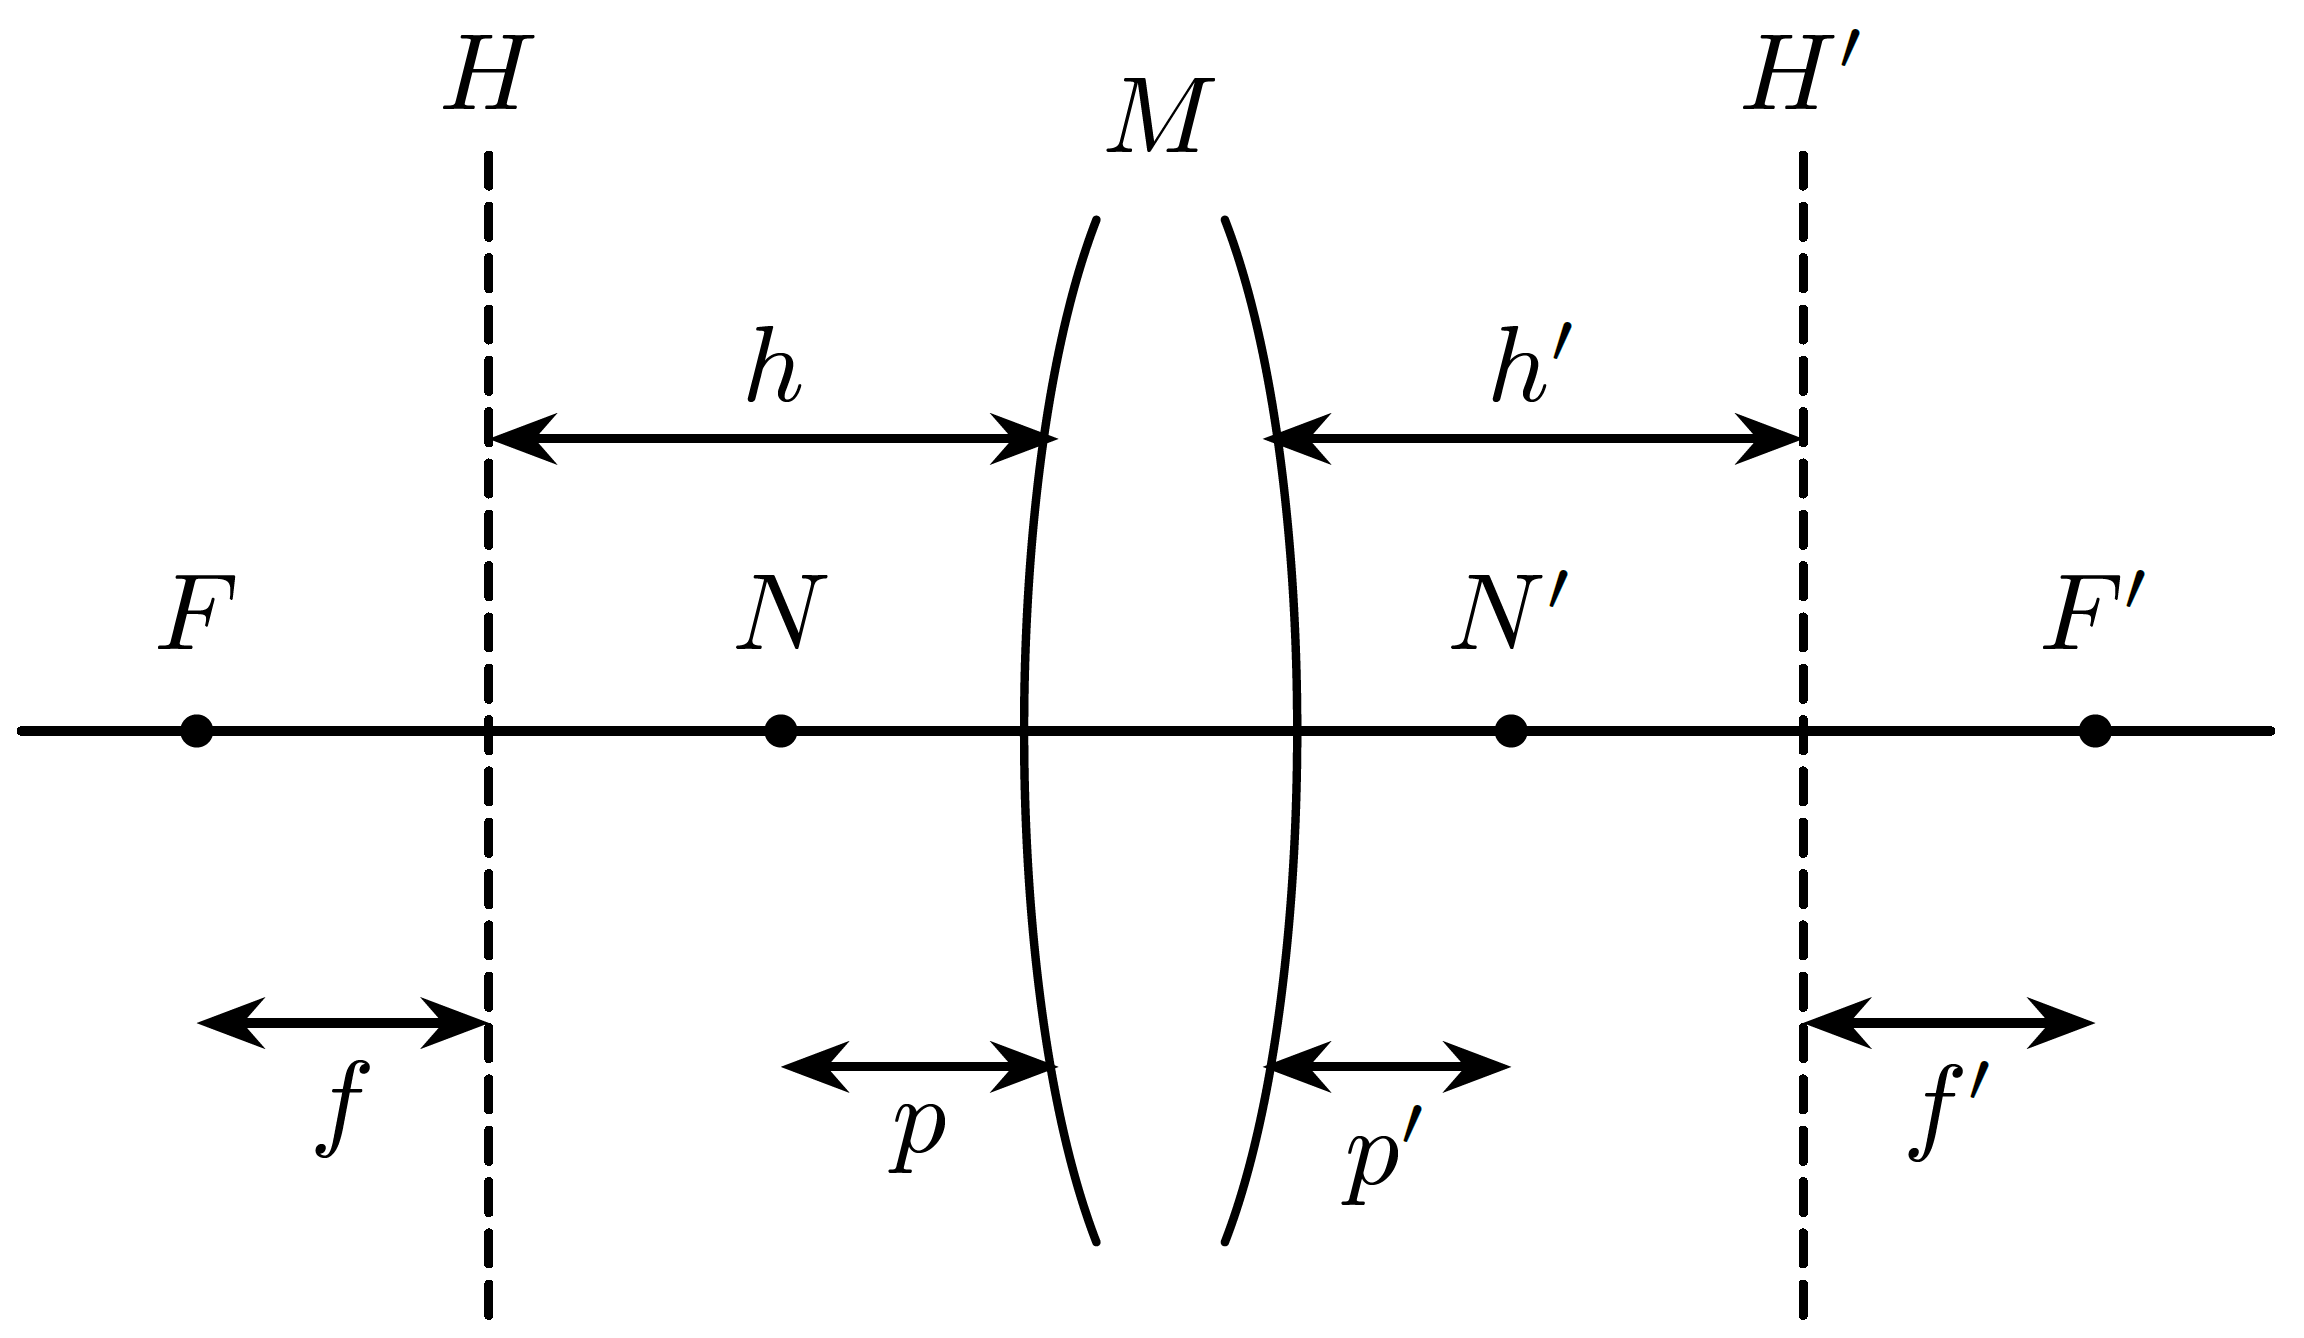
\includegraphics[width=\textwidth]{matrix_optics_fig/principal_planes_nodes_and_foci.png}
		\caption{主面\(H\)和\(H'\)、节点\(N\)和\(N'\)、焦点\(F\)和\(F'\)}
		\label{主面H和H'、节点N和N'、焦点F和F'}
		\label{主面节点焦点图}
	\end{minipage}
	\hfill
	\begin{minipage}[b]{0.53\textwidth}
		\centering
		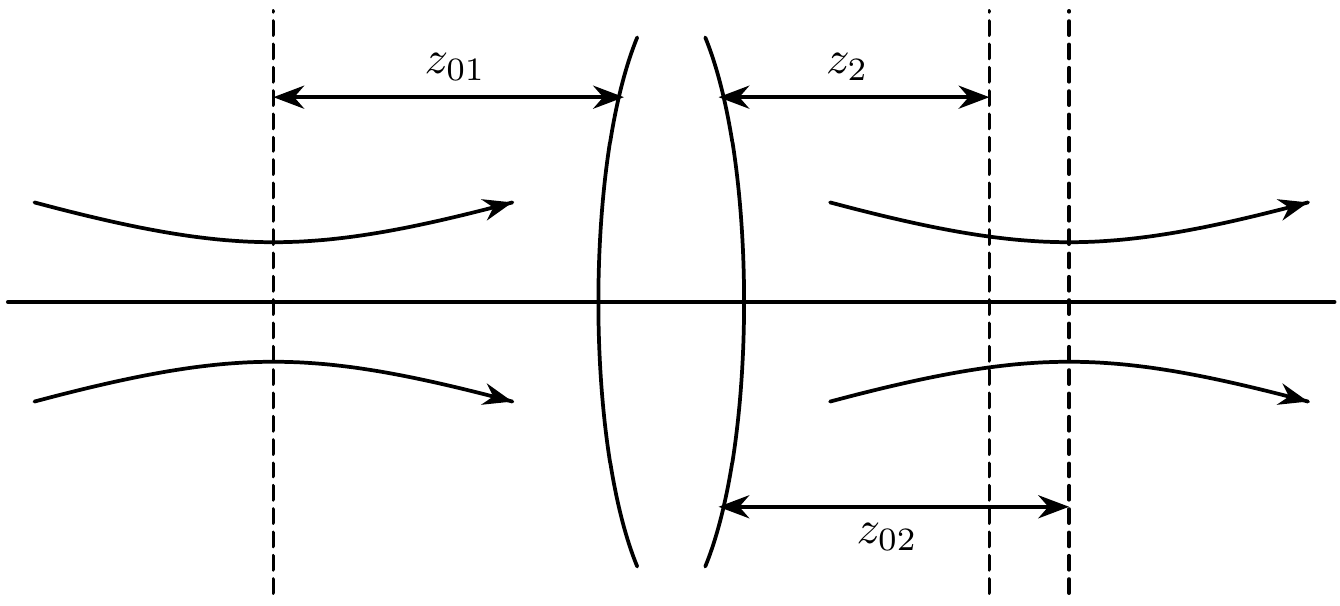
\includegraphics[width=\textwidth]{matrix_optics_fig/gaussian_beam_through_lens_group.png}
		\caption{高斯光束通过透镜组}
		\label{高斯光束通过透镜组}
	\end{minipage}
\end{figure}

根据矩阵光学理论，任意一束高斯光束经过理想光具组后仍具有高斯光束振幅、相位形式，证明如下：

引入复曲率半径 \(\rho(z)=z - \mathrm{i}q_0\)，则
\begin{equation*}
	\dfrac{1}{\rho(z)}=\dfrac{1}{R(z)}+\dfrac{2\mathrm{i}}{k\,\omega(z)^2},
\end{equation*}
并有
\begin{equation}
	U(r, z) =
	U_0 \cdot \dfrac{\omega_0}{\omega(z)} \cdot
	\exp\left[
		\mathrm{i}k\left(z + \dfrac{r^2}{2\rho(z)}\right)
		\right]
	\cdot \exp\left[ -\mathrm{i} \varphi(z) \right].
\end{equation}


进一步，高斯光束傍轴经过理想光具组可视为曲率半径为 \(\rho(z)\) 的发散球面波.

设某处前、后变换面波面的曲率半径分别为 \(\rho_1\)、\(\rho_2\)，入射光参数为 \((k_1,q_{01},\omega_{01})\)，记该处变换矩阵为
\begin{equation*}
	\begin{pmatrix}a'&b'\\c'&d'\end{pmatrix}.
\end{equation*}

根据定义及小角关系
\begin{equation*}
	\rho_1=\dfrac{y}{\alpha},\quad
	y'=a'y+b'\alpha,\quad
	\alpha'=c'y+d'\alpha,
\end{equation*}

解得
\begin{equation*}
	\rho_2=\dfrac{y'}{\alpha'}
	=\dfrac{a'\,\rho_1+b'}{c'\,\rho_1+d'}.
\end{equation*}

代入
\begin{equation*}
	\dfrac1{\rho_1}=\dfrac1{R_1}+\dfrac{2\mathrm{i}}{k_1\omega_1^2},\quad\dfrac1{\rho_2}=\dfrac1{R_2}+\dfrac{2\mathrm{i}}{k_2\omega_2^2}
\end{equation*}

得到
\begin{align*}
	R_2
	 & = \dfrac{
		\left( a' + \dfrac{b'}{R_1} \right)^2 +
		\left( \dfrac{2}{k_1 \omega_1^2} \right)^2 b'^2
	}{
		\left( a' + \dfrac{b'}{R_1} \right) \left( c' + \dfrac{d'}{R_1} \right) +
		\left( \dfrac{2}{k_1 \omega_1^2} \right)^2 b' d'
	},
	\quad\omega_2^2
	= \omega_1^2 \cdot \dfrac{k_1}{k_2} \cdot
	\dfrac{
		\left( a' + \dfrac{b'}{R_1} \right)^2 +
		\left( \dfrac{2}{k_1 \omega_1^2} \right)^2 b'^2
	}{
		a'd' - b'c'
	}.
\end{align*}


令该处的前变换面恰位于入射光束中心，即有\(R_1=\infty\)，假设该处距透镜组的前变换面\(z_{01}\)，该处后变换面距透镜组后变换面\(z_2\)，记透镜组的变换矩阵为
\begin{equation*}
	\begin{pmatrix}a&b\\c&d\end{pmatrix}.
\end{equation*}

进而
\begin{equation*}
	\begin{pmatrix}a'&b'\\c'&d'\end{pmatrix}
	=
	\begin{pmatrix}1 & z_2\\0 & 1\end{pmatrix}
	\begin{pmatrix}a & b\\c & d\end{pmatrix}
	\begin{pmatrix}1 & z_{01}\\0 & 1\end{pmatrix}
	=
	\begin{pmatrix}
		a+c\,z_2 & a\,z_{01}+b+z_2(c\,z_{01}+d) \\[4pt]
		c        & c\,z_{01}+d
	\end{pmatrix}.
\end{equation*}

代入得
\begin{align*}
	R_2
	 & =\dfrac{q_{01}^2(a+c\,z_2)^2+\bigl(b+a\,z_{01}+z_2(c\,z_{01}+d)\bigr)^2}
	{q_{01}^2\,c\,(a+c\,z_2)
	+\bigl(b+a\,z_{01}+z_2(c\,z_{01}+d)\bigr)(c\,z_{01}+d)},                    \\[4pt]
	\dfrac{k_2\omega_2^2}{2}
	 & =\dfrac{1}{q_{01}}
	\dfrac{q_{01}^2(a+c\,z_2)^2+\bigl(b+a\,z_{01}+z_2(c\,z_{01}+d)\bigr)^2}{ad-bc}.
\end{align*}

注意到，若记
\begin{equation*}
	q_{02}
	=\dfrac{q_{01}(ad-bc)}{q_{01}^2c^2+(c\,z_{01}+d)^2},\quad
	z_{02}
	=-\dfrac{q_{01}^2\,a\,c+(a\,z_{01}+b)(c\,z_{01}+d)}{q_{01}^2c^2+(c\,z_{01}+d)^2},
\end{equation*}
则上式可写为
\begin{equation}
	R_2=\dfrac{q_{02}^2+(z_2-z_{02})^2}{\,z_2-z_{02}\,},\quad
	\dfrac{k_2\omega_2^2}{2}
	=\dfrac{q_{02}^2+(z_2-z_{02})^2}{q_{02}}.
\end{equation}

可见，出射光仍为高斯光束（如图	\ref{高斯光束通过透镜组}），其共焦参量\(q_{02}\)、光束中心到透镜组后变换面的距离\(z_{02}\)如上.

另外注意到，若用透镜组的焦距和主面位置
\begin{equation*}
	f'=-\dfrac{1}{c},\quad
	f=-\dfrac{ad-bc}{c},\quad
	h'=\dfrac{1-a}{c},\quad
	h=\dfrac{ad-bc-d}{c}.
\end{equation*}
表示，则上式等价为
\begin{align*}
	 & z_{02}=h'+\dfrac{f'\,\bigl(q_{01}^2 - (z_{01}-h)(f - z_{01}+h)\bigr)}
	{q_{01}^2+(f - z_{01}+h)^2},\quad q_{02}=\dfrac{q_{01}\,f\,f'}{q_{01}^2+(f - z_{01}+h)^2}, \\[4pt]
	 & (z_{02}-f'-h')(z_{01}-f-h)=f\,f'\,\dfrac{(z_{01}-f-h)^2}{q_{01}^2+(z_{01}-f-h)^2},
\end{align*}

可见，入射与出射光束中心位置满足修正的牛顿成像关系，其在几何光学极限 \(q_{01}\to 0\) 下退化为牛顿成像定律.这是高斯光束经透镜组成像的又一特点.

